\documentclass[12pt]{article}
\usepackage[left=1cm, right=1cm, top=2cm,bottom=1.5cm]{geometry} 

\usepackage[parfill]{parskip}
\usepackage[utf8]{inputenc}
\usepackage[T2A]{fontenc}
\usepackage[russian]{babel}
\usepackage{enumitem}
\usepackage[normalem]{ulem}
\usepackage{amsfonts, amsmath, amsthm, amssymb, mathtools,xcolor,accents}
\usepackage{blkarray}

\usepackage{tabularx}
\usepackage{hhline}

\usepackage{accents}
\usepackage{fancyhdr}
\pagestyle{fancy}
\renewcommand{\headrulewidth}{1.5pt}
\renewcommand{\footrulewidth}{1pt}

\usepackage{graphicx}
\usepackage[figurename=Рис.]{caption}
\usepackage{subcaption}
\usepackage{float}

%%Наименование папки откуда забирать изображения
\graphicspath{ {./images/} }

%%Изменение формата для ввода доказательства
\renewcommand{\proofname}{$\square$  \nopunct}
\renewcommand\qedsymbol{$\blacksquare$}

%%Изменение отступа на таблицах
\addto\captionsrussian{%
	\renewcommand{\proofname}{$\square$ \nopunct}%
}
%% Римские цифры
\newcommand{\RN}[1]{%
	\textup{\uppercase\expandafter{\romannumeral#1}}%
}

%% Для удобства записи
\newcommand{\MR}{\mathbb{R}}
\newcommand{\MC}{\mathbb{C}}
\newcommand{\MQ}{\mathbb{Q}}
\newcommand{\MN}{\mathbb{N}}
\newcommand{\MZ}{\mathbb{Z}}
\newcommand{\MTB}{\mathbb{T}}
\newcommand{\MTI}{\mathbb{I}}
\newcommand{\MI}{\mathrm{I}}
\newcommand{\MCI}{\mathcal{I}}
\newcommand{\MJ}{\mathrm{J}}
\newcommand{\MH}{\mathrm{H}}
\newcommand{\MT}{\mathrm{T}}
\newcommand{\MU}{\mathcal{U}}
\newcommand{\MV}{\mathcal{V}}
\newcommand{\MA}{\mathcal{A}}
\newcommand{\MB}{\mathcal{B}}
\newcommand{\MF}{\mathcal{F}}
\newcommand{\ME}{\mathcal{E}}
\newcommand{\MW}{\mathcal{W}}
\newcommand{\ML}{\mathcal{L}}
\newcommand{\MP}{\mathcal{P}}
\newcommand{\VN}{\varnothing}
\newcommand{\VE}{\varepsilon}
\newcommand{\dx}{\, dx}
\newcommand{\dy}{\, dy}
\newcommand{\dz}{\, dz}
\newcommand{\dd}{\, d}


\theoremstyle{definition}
\newtheorem{defn}{Опр:}
\newtheorem{rem}{Rm:}
\newtheorem{prop}{Утв.}
\newtheorem{exrc}{Упр.}
\newtheorem{problem}{Задача}
\newtheorem{lemma}{Лемма}
\newtheorem{theorem}{Теорема}
\newtheorem{corollary}{Следствие}

\newenvironment{cusdefn}[1]
{\renewcommand\thedefn{#1}\defn}
{\enddefn}

\DeclareRobustCommand{\divby}{%
	\mathrel{\text{\vbox{\baselineskip.65ex\lineskiplimit0pt\hbox{.}\hbox{.}\hbox{.}}}}%
}
\DeclareRobustCommand{\ndivby}{\mkern-1mu\not\mathrel{\mkern4.5mu\divby}\mkern1mu}


%Короткий минус
\DeclareMathSymbol{\SMN}{\mathbin}{AMSa}{"39}
%Длинная шапка
\newcommand{\overbar}[1]{\mkern 1.5mu\overline{\mkern-1.5mu#1\mkern-1.5mu}\mkern 1.5mu}
%Функция знака
\DeclareMathOperator{\sgn}{sgn}

%Функция ранга
\DeclareMathOperator{\rk}{\text{rk}}
\DeclareMathOperator{\diam}{\text{diam}}


%Обозначение константы
\DeclareMathOperator{\const}{\text{const}}

\DeclareMathOperator{\codim}{\text{codim}}

\DeclareMathOperator*{\dsum}{\displaystyle\sum}
\newcommand{\ddsum}[2]{\displaystyle\sum\limits_{#1}^{#2}}
\newcommand{\ddssum}[2]{\displaystyle\smashoperator{\sum\limits_{#1}^{#2}}}
\newcommand{\ddlsum}[2]{\displaystyle\smashoperator[l]{\sum\limits_{#1}^{#2}}}
\newcommand{\ddrsum}[2]{\displaystyle\smashoperator[r]{\sum\limits_{#1}^{#2}}}

%Интеграл в большом формате
\DeclareMathOperator{\dint}{\displaystyle\int}
\newcommand{\ddint}[2]{\displaystyle\int\limits_{#1}^{#2}}
\newcommand{\ssum}[1]{\displaystyle \sum\limits_{n=1}^{\infty}{#1}_n}

\newcommand{\smallerrel}[1]{\mathrel{\mathpalette\smallerrelaux{#1}}}
\newcommand{\smallerrelaux}[2]{\raisebox{.1ex}{\scalebox{.75}{$#1#2$}}}

\newcommand{\smallin}{\smallerrel{\in}}
\newcommand{\smallnotin}{\smallerrel{\notin}}

\newcommand*{\medcap}{\mathbin{\scalebox{1.25}{\ensuremath{\cap}}}}%
\newcommand*{\medcup}{\mathbin{\scalebox{1.25}{\ensuremath{\cup}}}}%

\makeatletter
\newcommand{\vast}{\bBigg@{3.5}}
\newcommand{\Vast}{\bBigg@{5}}
\makeatother

%Промежуточное значение для sup\inf, поскольку они имеют разную высоту
\newcommand{\newsup}{\mathop{\smash{\mathrm{sup}}}}
\newcommand{\newinf}{\mathop{\mathrm{inf}\vphantom{\mathrm{sup}}}}

%Скалярное произведение
\newcommand{\inner}[2]{\left\langle #1, #2 \right\rangle }
\newcommand{\linsp}[1]{\left\langle #1 \right\rangle }
\newcommand{\linmer}[2]{\left\langle #1 \vert #2\right\rangle }

%Подпись символов снизу
\newcommand{\ubar}[1]{\underaccent{\bar}{#1}}

%%Шапка для букв сверху
\newcommand{\wte}[1]{\widetilde{#1}}
\newcommand{\wht}[1]{\widehat{#1}}
\newcommand{\ovl}[1]{\overline{#1}}


%%Трансформация Фурье
\newcommand{\fourt}[1]{\mathcal{F}\left(#1\right)}
\newcommand{\ifourt}[1]{\mathcal{F}^{-1}\left(#1\right)}

%%Символ вектора
\newcommand{\vecm}[1]{\overrightarrow{#1\,}}

%%Пространстов матриц
\newcommand{\matsq}[1]{\operatorname{Mat}_{#1}}
\newcommand{\mat}[2]{\operatorname{Mat}_{#1, #2}}

%Оператор для действ и мнимых чисел
\DeclareMathOperator{\IM}{\operatorname{Im}}
\DeclareMathOperator{\RE}{\operatorname{Re}}
\DeclareMathOperator{\li}{\operatorname{li}}
\DeclareMathOperator{\GL}{\operatorname{GL}}
\DeclareMathOperator{\SL}{\operatorname{SL}}
\DeclareMathOperator{\Char}{\operatorname{char}}
\DeclareMathOperator\Arg{Arg}
\DeclareMathOperator\ord{ord}

%Оператор для образа
\DeclareMathOperator{\Ima}{Im}

%Делимость чисел
\newcommand{\modn}[3]{#1 \equiv #2 \; (\bmod \; #3)}
\newcommand{\nmodn}[3]{#1 \not\equiv #2 \; (\bmod \; #3)}

%%Взятие в скобки, модули и норму
\newcommand{\parfit}[1]{\left( #1 \right)}
\newcommand{\modfit}[1]{\left| #1 \right|}
\newcommand{\sqparfit}[1]{\left\{ #1 \right\}}
\newcommand{\normfit}[1]{\left\| #1 \right\|}

%%Функция для обозначения равномерной сходимости по множеству
\newcommand{\uconv}[1]{\overset{#1}{\rightrightarrows}}
\newcommand{\uconvm}[2]{\overset{#1}{\underset{#2}{\rightrightarrows}}}

%% Функция для добавления круга сверху множества
\newcommand{\Circ}[1]{\accentset{\circ}{#1}}

%%Функция для обозначения нижнего и верхнего интегралов
\def\upint{\mathchoice%
	{\mkern13mu\overline{\vphantom{\intop}\mkern7mu}\mkern-20mu}%
	{\mkern7mu\overline{\vphantom{\intop}\mkern7mu}\mkern-14mu}%
	{\mkern7mu\overline{\vphantom{\intop}\mkern7mu}\mkern-14mu}%
	{\mkern7mu\overline{\vphantom{\intop}\mkern7mu}\mkern-14mu}%
	\int}
\def\lowint{\mkern3mu\underline{\vphantom{\intop}\mkern7mu}\mkern-10mu\int}

%%След матрицы
\DeclareMathOperator*{\tr}{tr}

\makeatletter
\renewcommand*\env@matrix[1][*\c@MaxMatrixCols c]{%
	\hskip -\arraycolsep
	\let\@ifnextchar\new@ifnextchar
	\array{#1}}
\makeatother


%% Переопределение функции хи, чтобы выглядела более приятно
\makeatletter
\@ifdefinable\@latex@chi{\let\@latex@chi\chi}
\renewcommand*\chi{{\@latex@chi\smash[t]{\mathstrut}}} % want only bottom half of \mathstrut
\makeatletter

\setcounter{MaxMatrixCols}{20}

\begin{document}
\lhead{Математический анализ - \RN{4}}
\chead{Шапошников С.В.}
\rhead{Лекция - 12}
\section*{Меры. Внешние меры}

\subsection*{Мера Лебега}
\begin{prop}
	$$
		E \subset \MA_\lambda \Leftrightarrow E = \bigcup\limits_m K_m \cup E_0 \Leftrightarrow E = B \cup B_0
	$$ 
	где $K_m$ это компакты, $E_0$ и $B_0$ это множества меры нуль и $B$ это борелевское множество.
\end{prop}

\begin{proof}\hfill
	\begin{enumerate}[label=\arabic*)]
		\item Покажем, что всякое борелевское множество $B$ можно представить в виде $B = \cup_m K_m \cup B_0$, где $K_m$ это компакты, $B_0$ это множество меры нуль. Можно считать, что $B \subset \MI$ - лежит в некотором замкнутом бруске, поскольку всё $\MR^n$ можно представить в виде счетного объединения замкнутых брусов, тогда:
		$$
			\MR^n = \bigcup\limits_k \MI_k \Rightarrow B = \bigcup\limits_k (\MI_k \cap B)
		$$
		Следовательно, если каждое множество $\MI_k \cap B$ представить в виде счетного объединения компактов и счетного множества меры нуль (что просто будет множеством меры нуль), то можно и всё борелевское так представить. $\lambda$ это конечная $\sigma$-аддитивная мера на борелевских множествах на бруске: $\MB(\MI)$, тогда по теореме с прошлой лекции будет верно:
		$$
			\forall m, \, \exists \, F_m \subset B \colon \lambda(B \setminus F_m) < \dfrac{1}{m}
		$$
		$F_m$ это замкнутое множество, $F_m \subset \MI \Rightarrow F_m$ это компакт. Возьмем объединение $F_m$, тогда:
		$$
			\bigcup\limits_m F_m \subset B , \, B \setminus \bigcup\limits_m F_m \subset B \setminus F_m \Rightarrow \lambda(B \setminus \cup_m F_m) \leq \lambda(B \setminus F_m) < \dfrac{1}{m} \to 0
		$$
		Следовательно, получаем: 
		$$
			B = \bigcup\limits_m F_m \cup \left(B \setminus \bigcup\limits_m F_m\right)
		$$ 
		где $B \setminus \cup_m F_m$ это множество меры нуль;
		\item Заметим, что все стрелочки $\Leftarrow$ очевидны, поскольку борелевские множества - измеримы $\Rightarrow$ компакты измеримы, мы знаем, что множества меры нуль всегда измеримы (в самом начале обсуждения внешней меры проговорили) и также мы знаем, что множество измеримых это $\sigma$-алгебра $\Rightarrow$ всё что получаем счётным объединением это элемент этой $\sigma$-алгебры;
		\item По первому пункту достаточно доказать, что всякое измеримое множество $E$ есть объединение борелевского с множеством меры нуль. Разберём случай, когда $E$ лежит в брусе $\MI$: $E \subset \MI$ по аналогичным с пунктом $1)$ причинам. Рассмотрим множество $D = \MI \setminus E$, это измеримое по Лебегу множество, как разница двух измеримых, тогда:
		$$
			\exists \, \{\MI_j^m\} \colon D \subset \bigcup\limits_j \MI_j^m = D_m, \,  \ddsum{j}{}|\MI_j^m| \leq \lambda(D) + \dfrac{1}{m}
		$$
		где последнее верно в силу того, что мы выбрали покрытие, которое мало отличается от точной нижней грани по $D$. Заметим, что  $D_m$ это борелевское множество, как счетное объединение борелевских множеств, кроме того $D \subset D_m$ и верно:
		$$
			\lambda(D_m) \leq \ddsum{j}{}|\MI_j^m| \leq \lambda(D) + \dfrac{1}{m}, \, D \subset D_m \Rightarrow  \lambda(D_m \setminus D) = \lambda(D_m) - \lambda(D \cap D_m)  \leq \dfrac{1}{m}
		$$
		Рассмотрим $C = \cap_m D_m$, это опять борелевское множество, более того, $\forall m, \, D\subset D_m \Rightarrow D \subset C$. Заметим также, что верно:
		$$
			C \subset D_m \Rightarrow (C \setminus D) \subset (D_m \setminus D) \Rightarrow \lambda(C \setminus D) \leq \lambda(D_m \setminus D) \leq \dfrac{1}{m} \xrightarrow[m \to \infty]{} 0
		$$
		Устремляя $m \to \infty$, мы получаем, что $\lambda(C \setminus D) = 0$. Таким образом, мы взяли дополнение к $E$ и накрыли его борелевским множеством, которое отличается по мере от множества $D$ на множество меры нуль $\Rightarrow$ мы представили $D$ как борелевское множество минус множество меры нуль. Рассмотрим множество $B = \MI \setminus C$, тогда: $B \subset E$, $B$ - борелевское.
		\begin{figure}[H]
			\centering
			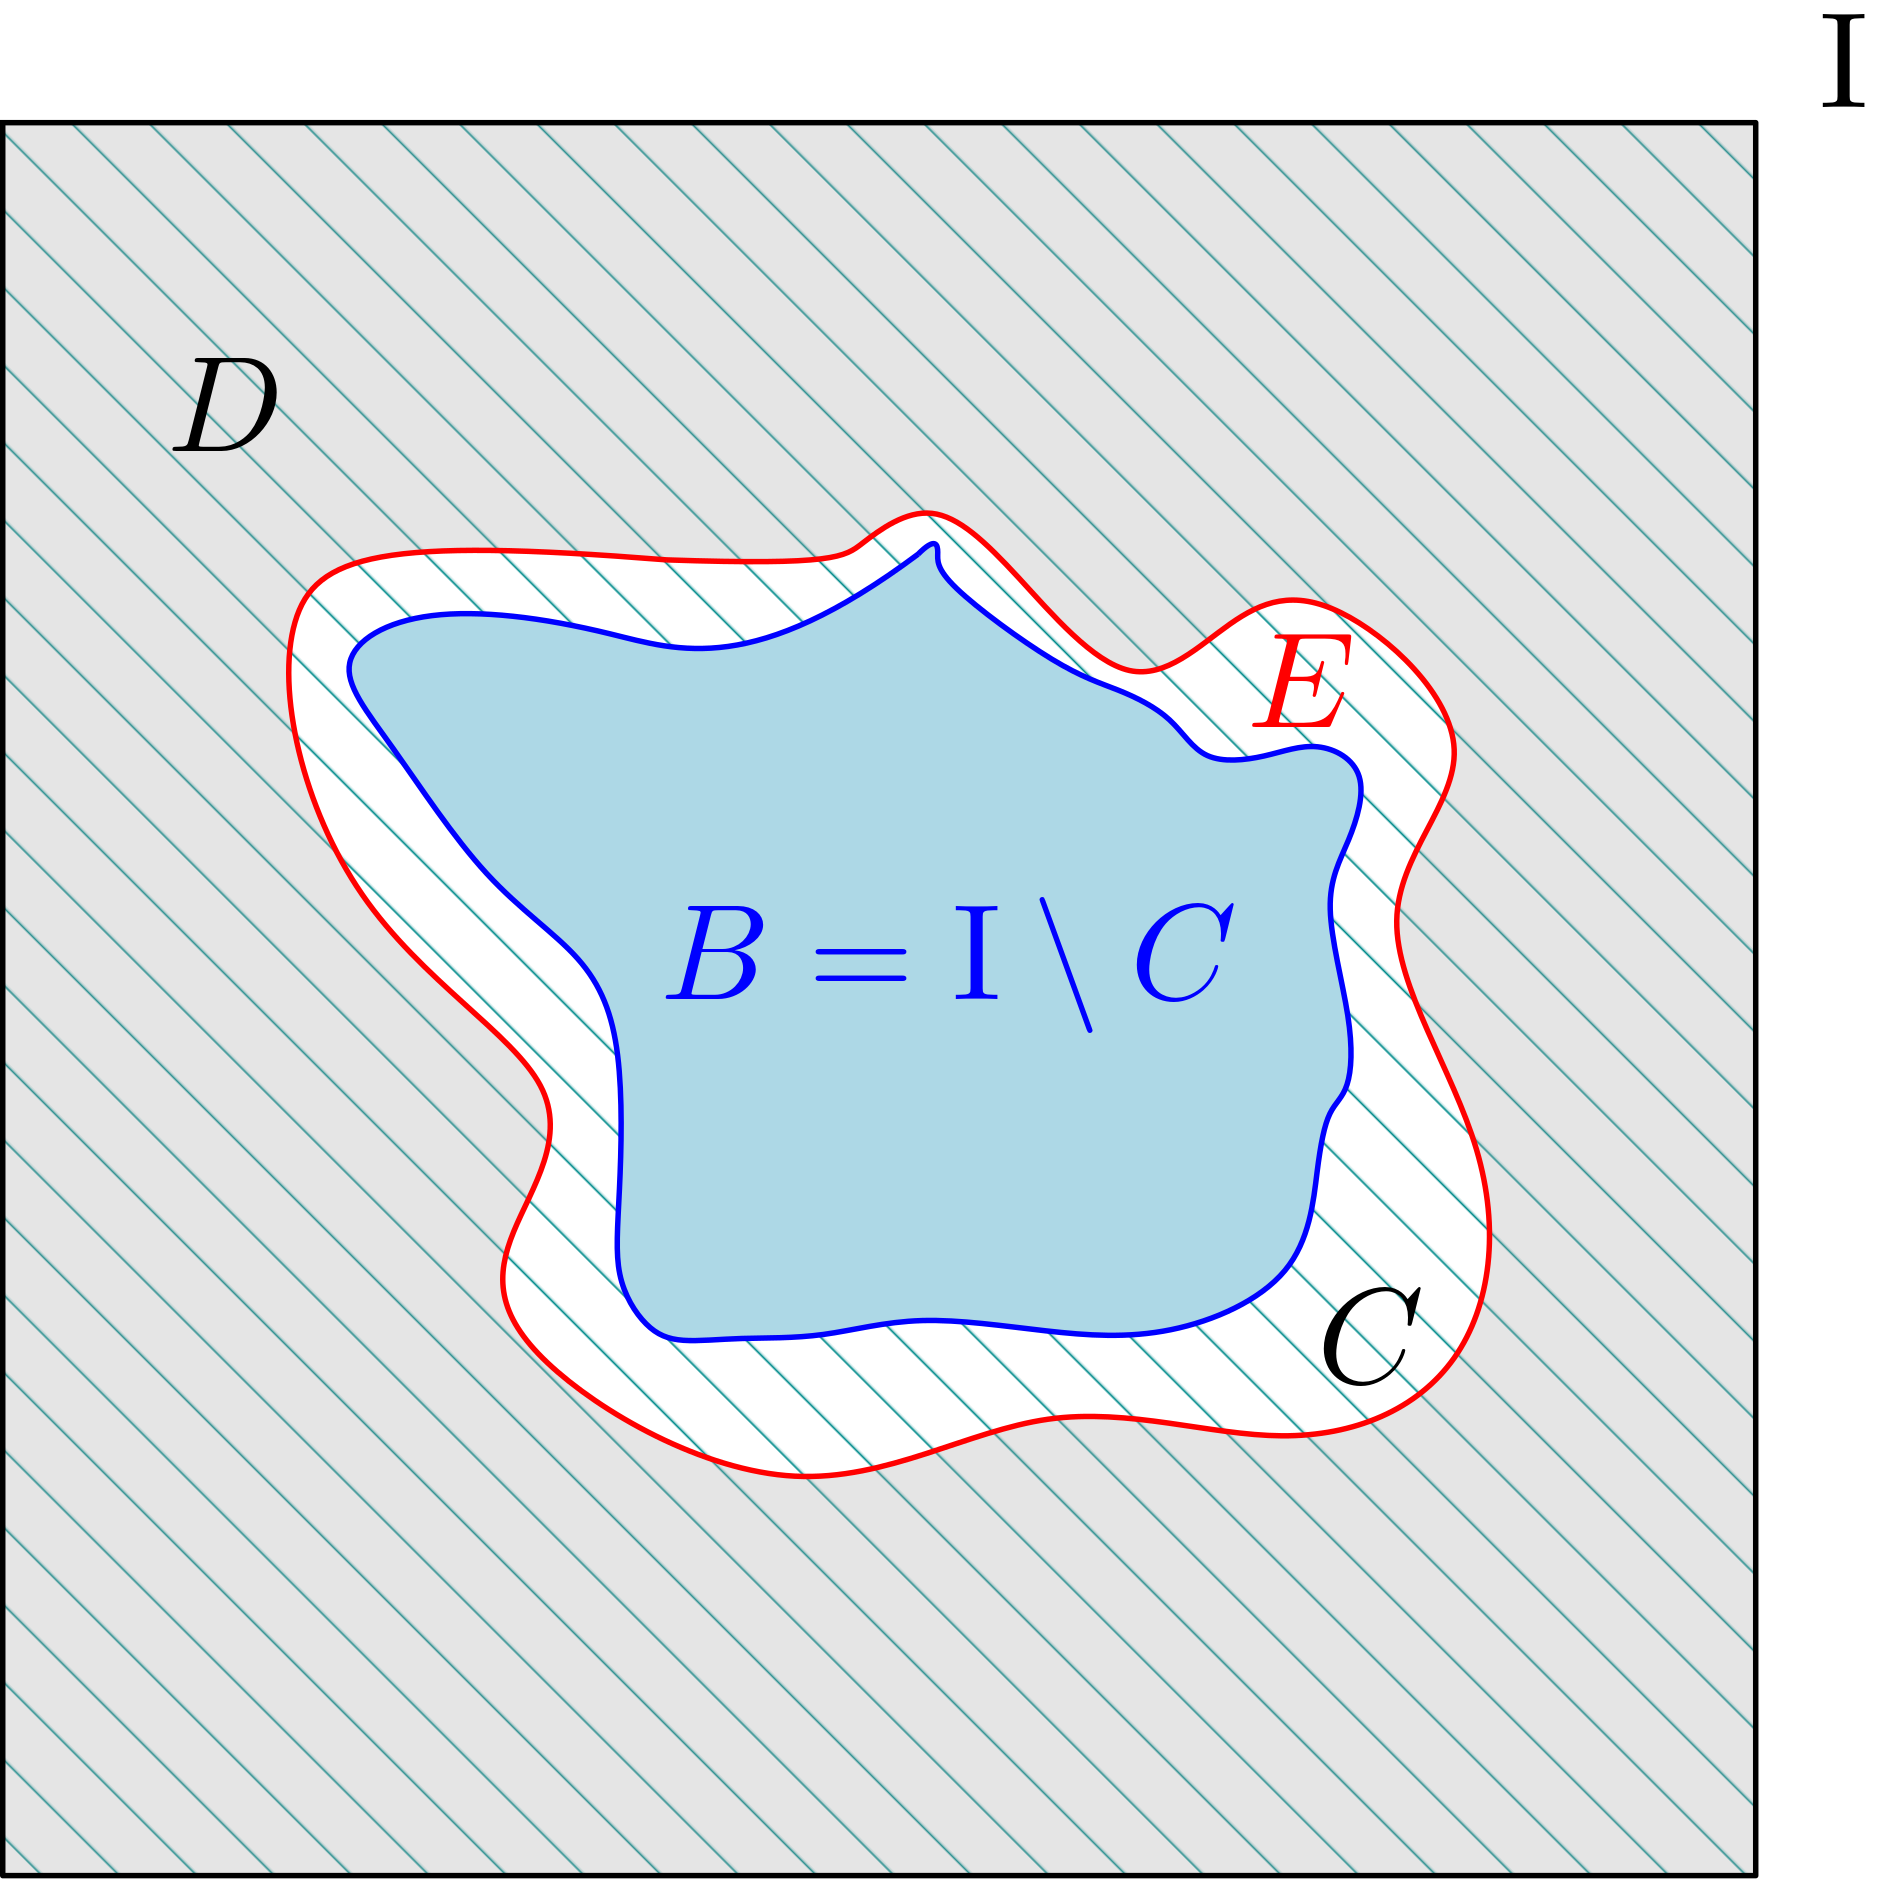
\includegraphics[width=0.3\textwidth]{MA4L12_1.png}
			\caption{Построение множества $B$.}
			\label{12_1}
		\end{figure}
		Также заметим, что: $E \setminus B = C \setminus D$ или подробнее: 
		$$
			E \setminus B = E \setminus( \MI \setminus C) = (E \cap C) \cup (E \setminus \MI) = E \cap C = (C \cap E) \cup (C \setminus \MI)= C \setminus (\MI \setminus E) = C \setminus D \Rightarrow
		$$
		$$
			\Rightarrow \lambda(E \setminus B) = \lambda(C \setminus D ) = 0 \Rightarrow E = B \cup (E \setminus B) = B \cup B_0
		$$
		Итого, $E$ это борелевское множество $B$ объединенное с множеством меры нуль $B_0 = E\setminus B$;
	\end{enumerate}
\end{proof}
\begin{rem}
	Фактически в последнем пункте доказательства мы взяли измеримое множество $D$ и поместили его в борелевское множество $C$ так, что зазор оказался меры нуль: $\lambda(C \setminus D) = 0$. Следовательно, переходя к дополнениям мы научились включать внутрь борелевское множество так, чтобы зазор был меры нуль.
\end{rem}

\begin{corollary}
	Пусть $f \colon \MR^m \to \MR^n, \, n \geq m$ - локально липшицево отображение, то есть на каждом брусе верно: 
	$$
		\exists \, L > 0 \colon \|f(x_1) - f(x_2)\| \leq L{\cdot}\|x_1 - x_2\|
	$$
	Тогда для всякого измеримого по Лебегу множества $E \subset \MR^m$ множество $f(E)$ измеримо.
\end{corollary}
\begin{proof}
	Ранее уже было доказано (см. лекцию $6$), что если $E$ это множество меры нуль, то $f(E)$ это множество меры нуль. Пусть $E$ - произвольное измеримое множество, тогда по утверждению выше:
	$$
		E = \bigcup\limits_s K_s \cup A, \, \lambda(A) = 0 \Rightarrow f(E) = \bigcup\limits_s f(K_s) \cup f(A)
	$$
	Поскольку отображение локально липшицево, то образ компакта - компакт, а $f(A)$ это множество меры нуль, следовательно $f(E)$ это измеримое множество.
\end{proof}
\begin{rem}
	Множество меры нуль не обязательно будет переходить в множество меры нуль. Например, функция: $\tfrac{C(x) + x}{2}$, где $C(x)$ - Канторовская лестница, есть гомеоморфизм $[0,1] \to [0,1]$ и это отображение множество Кантора переводит в множество меры $\tfrac{1}{2}$.
\end{rem}

\begin{rem}
	Аналогично с помощью отображения выше можно изготовить измеримое по Лебегу, но не Борелевское множество: в множестве положительной меры можно найти неизмеримое по Лебегу (множество Витали) и затем взять прообраз $\Rightarrow$ получится множество, которое будет лежать внутри Канторовского, но оно меры нуль $\Rightarrow$ всё что лежит внутри тоже меры нуль $\Rightarrow$ измеримо по Лебегу, но при этом это будет не Борелевское множество, поскольку при гомеоморфизме если получили Борелевское, то и было взято Борелевское.
\end{rem}
\begin{prop}
	Если $E$ это допустимое множество, то $E$ измеримо по Лебегу и $\lambda(E) = |E|$.
\end{prop}
\begin{proof}
	$E$ допустимое $\Rightarrow$ оно ограничено и $\partial E$ это множество меры нуль, тогда:
	$$
		E = \Circ{E} \cup A, \, A \subset \partial E \Rightarrow \lambda(A) = 0
	$$
	где мы берём $A$, поскольку $\partial E$ не обязательно принадлежит $E \Rightarrow E$ - измеримо. Заметим, что: 
	\begin{enumerate}[label=\arabic*)]
		\item $\ovl{E} = E \cup \partial E$ это допустимое множество, поскольку $E$ - допустимое и $\partial E$ - множество меры нуль. Ещё можно сказать так: $\partial E$ - это допустимое множество, поскольку граница границы это она сама (граница это замкнутое множество), а объединение допустимых это допустимое множество;
		\item $|E| = |\ovl{E}|$, это так поскольку эти множества отличаются на множество, объем которого равен нулю: $C \subset \partial E$, так как $\partial E$ - замкнутое множество, то $\partial C \subset \partial E$, поскольку замыкание - наименьшее замкнутое множество, содержащее $C$, $\partial E$ - ограниченное множество, так как $E$ - ограниченное $\Rightarrow C$ - ограниченное, $\partial C \subset \partial E \Rightarrow \partial C$ имеет меру нуль $\Rightarrow C$ это допустимое множество. Тогда: 
		$$
			\ovl{E} = E \cup C, \, C = \ovl{E}\setminus E \subset \partial E, \, E \cap C = \VN \Rightarrow |\ovl{E}| = |E \cup C| = |E| + |C| = |E|
		$$
		\item $\lambda(E) = \lambda(\ovl{E})$ - очевидно:
		$$
			\ovl{E} = E \cup C, \, C = \ovl{E}\setminus E \Rightarrow \lambda(\ovl{E}) = \lambda(\ovl{E}\setminus E) + \lambda(E \cap \ovl{E}) = \lambda(C) + \lambda(E) = \lambda(E)
		$$
	\end{enumerate}
	Далее, считаем, что $E$ - замкнуто. 
	\begin{figure}[H]
		\centering
		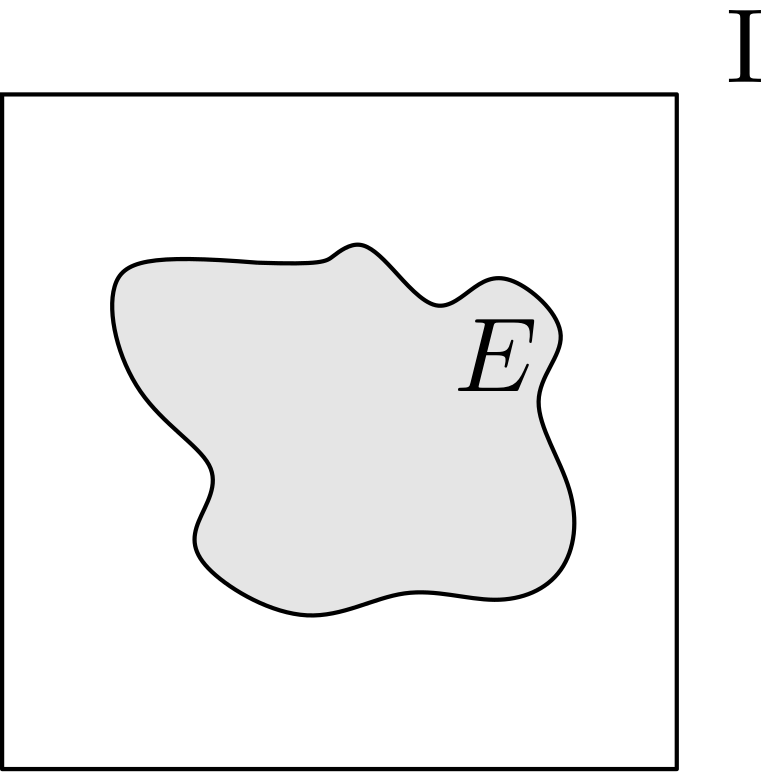
\includegraphics[width=0.2\textwidth]{MA4L12_2.png}
		\caption{Объем допустимого множества по определению внутри бруса $\MI$.}
		\label{12_2}
	\end{figure}
	По определению:
	$$
		\exists\, \MI \colon E \subset \MI, \, |E| = \ddint{\MI}{}\chi_E(x)dx
	$$
	Возьмем разбиение $\MTB_N = \{\MI_j^N\}$ бруска $\MI$ такое, что:
	\begin{enumerate}[label=(\arabic*)]
		\item $\diam\{\MI_j^N\} < \tfrac{1}{N}$;
		\item Каждое следующее разбиение $\MTB_{N+1}$ получается разбиением предыдущих брусков $\MTB_N$;
	\end{enumerate}
	\begin{figure}[H]
		\centering
		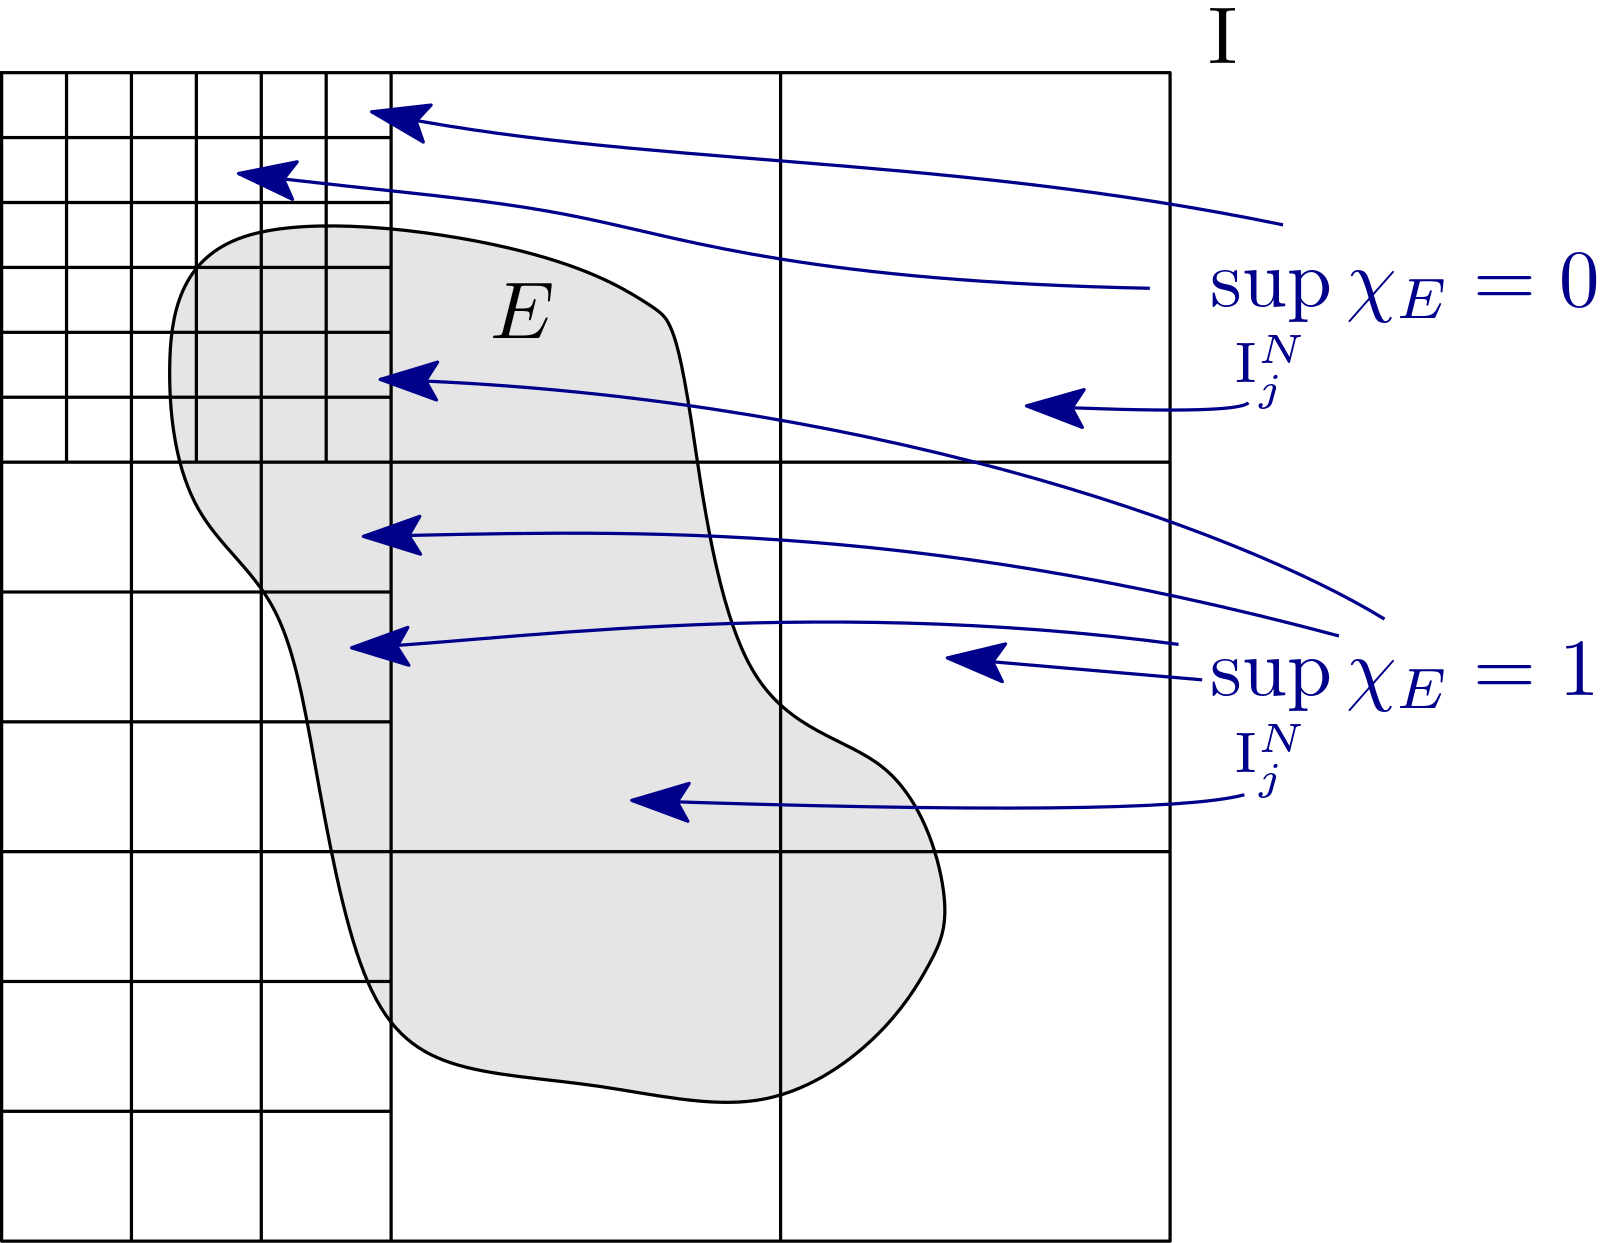
\includegraphics[width=0.35\textwidth]{MA4L12_3.png}
		\caption{Разбиение $\MTB_{N+1}$, полученное из предыдущего разбиения $\MTB_{N}$.}
		\label{12_3}
	\end{figure}
	Тогда будет верно:
	$$
		|E| = \lim\limits_{N \to \infty}\ddsum{j}{}\sup\limits_{\MI_j^N}\chi_E(x){\cdot}|\MI_j^N|, \quad \sup\limits_{\MI_j^N}\chi_E(x) = 
		\begin{cases}
			0, & \MI_j^N \cap E = \VN\\
			1, & \MI_j^N \cap E \neq \VN
		\end{cases}
	$$
	Рассмотрим объединение брусков разбиения пересекающихся с $E$: 
	$$
		Q_N = \bigcup\limits_{j \colon \MI_j^N \cap E \neq \VN}\MI_j^N \Rightarrow \lambda(Q_N) = \ddsum{j \colon \MI_j^N \cap E \neq \VN}{}|\MI_j^N| = \ddsum{j}{}\sup\limits_{\MI_j^N}\chi_E(x){\cdot}|\MI_j^N|
	$$
	\begin{figure}[H]
		\centering
		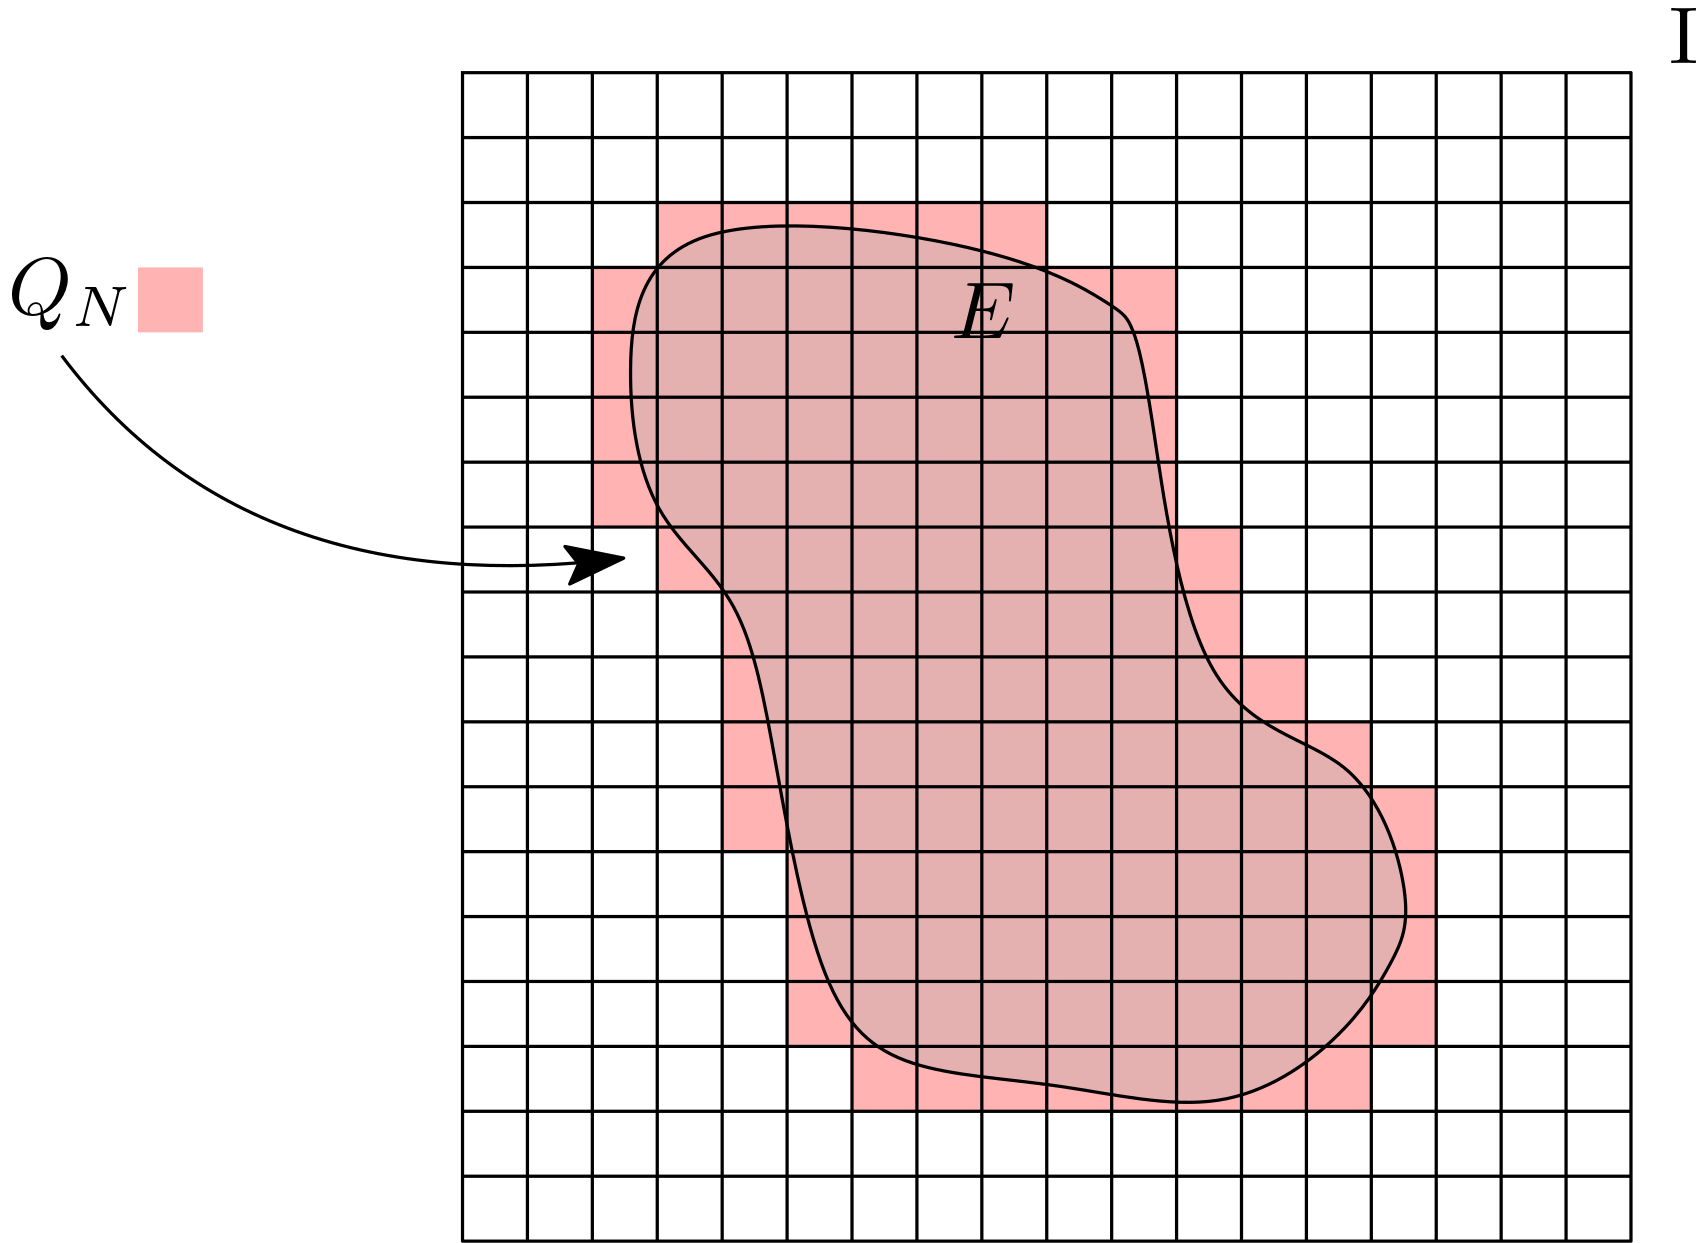
\includegraphics[width=0.4\textwidth]{MA4L12_4.png}
		\caption{Объединение брусков разбиения пересекающихся с $E$: $Q_N$.}
		\label{12_4}
	\end{figure}
	Заметим, что:
	$$
		\MI_j^{N+1} \cap E \neq \VN \Rightarrow\MI_j^{N+1} \subset \MI_k^N \Rightarrow \MI_k^N  \cap E \neq \VN \Rightarrow Q_{N+1}\subset Q_N
	$$ 
	\begin{figure}[H]
		\centering
		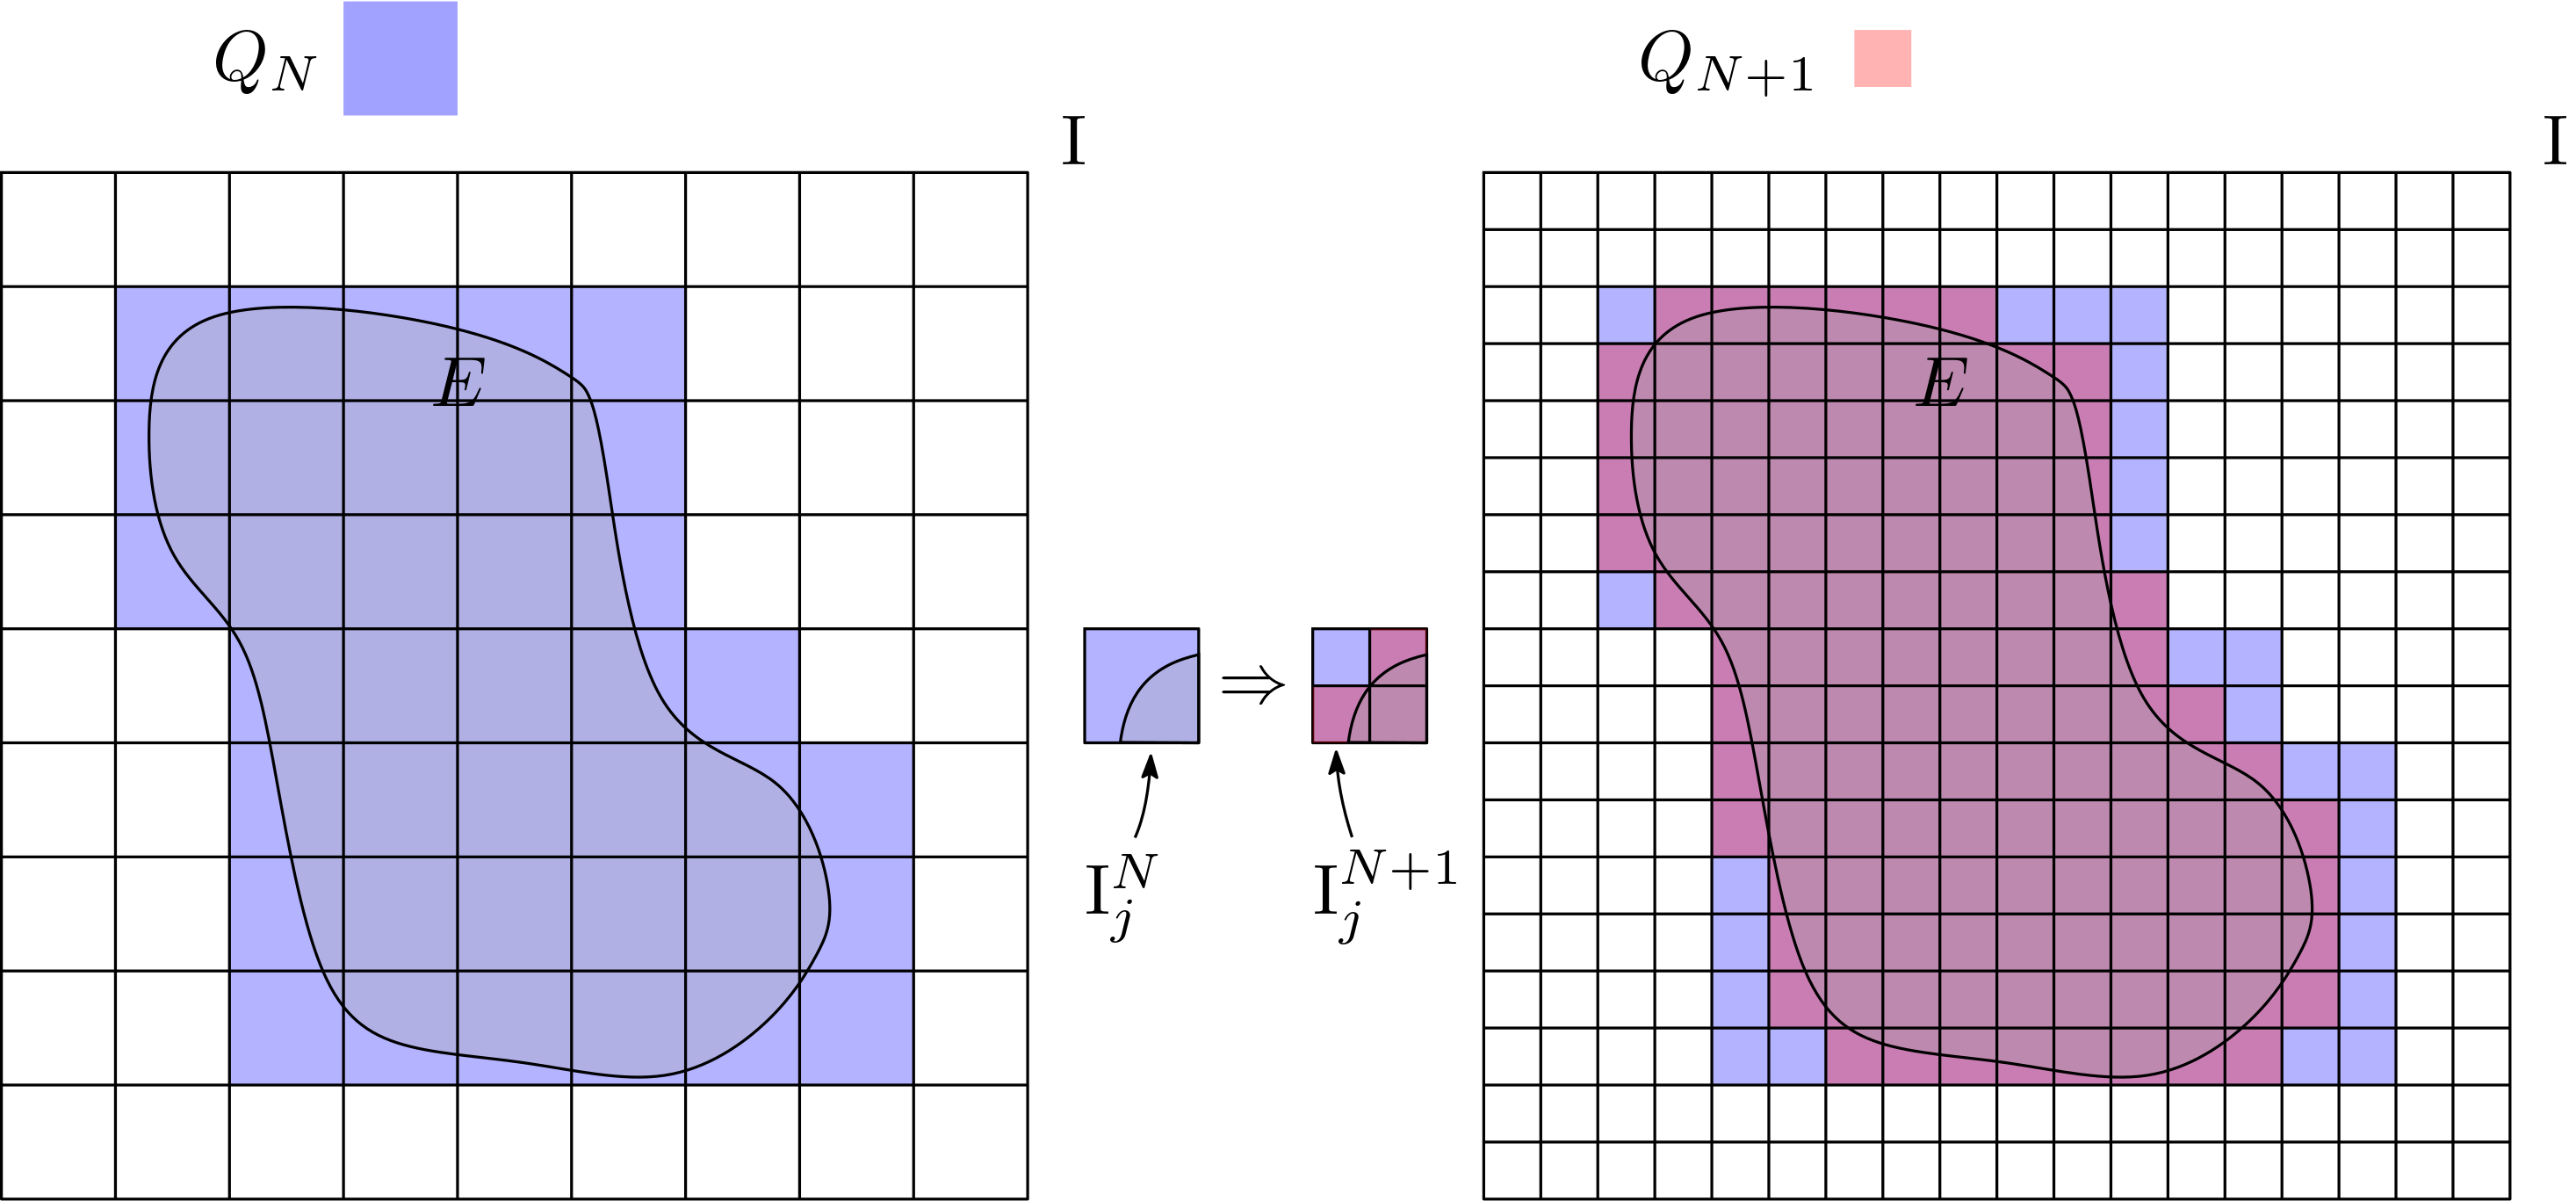
\includegraphics[width=0.7\textwidth]{MA4L12_5.png}
		\caption{Измельчение разбиения и влияние на $Q_N \colon Q_{N+1}\subset Q_N$.}
		\label{12_5}
	\end{figure}
	Кроме того $\cap_N Q_N = E$, поскольку очевидно, что: $\forall N, \, E \subset Q_N \Rightarrow E \subset \cap_N Q_N$. Пусть $\exists \, y \not\in E$ и $y \in \cap_N Q_N$, поскольку $E$ - замкнутое подмножество бруска $\MI$ (дополнение к замкнутому - открытое), тогда:
	$$
		\exists \, \MB(y,r) \subset \MI \colon \MB(y,r) \cap E = \VN \Rightarrow \exists \, N \colon \diam{\MI_j^N} < \dfrac{1}{N} < r 
	$$
	следовательно, никакой брусок разбиения не сможет задевать точку $y$, иначе внутри этого шара появилась бы точка множества $E \Rightarrow \cap_N Q_N = E$. Тогда по непрерывности меры:
	$$
		\ddsum{j}{}\sup\limits_{\MI_j^N}\chi_E(x){\cdot}|\MI_j^N| = \lambda(Q_N) \xrightarrow[N \to \infty]{}\lambda(E) \Rightarrow |E| = \lim\limits_{N \to \infty}\ddsum{j}{}\sup\limits_{\MI_j^N}\chi_E(x){\cdot}|\MI_j^N| = \lambda(E)
	$$
\end{proof}
Следствием этого утверждения является очень важная для нас теорема.

\begin{theorem}
	Пусть $L(x) = Ax + b$, где $A \in \mat{n}{n}$, $b$ - вектор. Тогда для всякого измеримого ограниченного множества $E$ верно равенство:
	$$
		\lambda(L(E)) = |\det{A}|{\cdot}\lambda(E)
	$$
\end{theorem}
\begin{rem}
	Заметим, что ограниченность нужна в случае, когда у нас бесконечность, а матрица $A$ - вырожденная, тогда надо будет пояснять, что в $0{\cdot}\infty$ ответом будет $0$.
\end{rem}
\begin{proof}
	Пусть $\det{A} = 0$, тогда $L(\MR^n)$ это подмножество гиперплоскости $\Rightarrow$ множество меры нуль. Подробнее:
	$$
		\left\{
		\begin{matrix}
			y_1 &= & a_{11}x_1 & + & \dotsc & + & a_{1n}x_n & + & b_1 \\
			\vdots & \vdots & \vdots & \vdots & \ddots & \vdots & \vdots & \vdots & \vdots \\
			y_n &= & a_{n1}x_1 & + & \dotsc & + & a_{nn}x_n & + & b_n
		\end{matrix}\right.
	$$
	Поскольку $\det{A} = 0$, то строчки линейно зависимы, тогда:
	$$
		\exists \, c_2, \dotsc, c_n  \colon y_1 - c_2y_2 - \dotsc - c_n y_n = \wte{b} \Rightarrow y_1 = c_2y_2 + \dotsc + c_n y_n + \wte{b}
	$$
	Мы получили уравнение, задающее гиперплоскость, или по-другому: всё что лежит на графике хорошей непрерывной функции это всё множество меры нуль, поскольку сам этот график является множеством меры нуль (см. лекцию $3$). Следовательно, получили верное равенство: $\lambda(L(\MR^n)) = 0 = 0{\cdot}\lambda(E)$.
	
	Пусть $\det{A} \neq \VN$, поскольку $E$ - ограниченное, то можно далее считать, что $E\subset \MI$ и рассматриваем только подмножества замкнутого бруса $\MI$. На измеримых по Лебегу множествах в бруске $\MI$ определены две $\sigma$-аддитивные, конечные меры: 
	$$
		\mu_1(E) = \lambda(L(E)), \quad \mu_2(E) =|\det{A}|{\cdot}\lambda(E)
	$$
	$L$ - линейное отображение $\Rightarrow$ локально липшицево (даже вообще липшицево) $\Rightarrow L(E)$ это измеримое множество. Для $\mu_2$ $\sigma$-аддитивность очевидна, поскольку $\det{A} \neq 0$ и мы просто умножаем на число. Для $\mu_1$ мы знаем, что $L$ это взаимнооднозначное соответствие, тогда:
	$$
		L(\cup_j E_j) = \cup_j L(E_j), \quad L(\cap_j E_j) = \cap_j L(E_j), \quad L(E \setminus D) = L(E) \setminus L(D)
	$$
	Следовательно, когда будем брать объединение попарно непересекающихся множеств, то сможем его выносить наружу и далее воспользоваться $\sigma$-аддитивностью $\lambda$ и обратно расставить $L \Rightarrow \mu_1$ тоже будет $\sigma$-аддитивной мерой. Заметим, ряд моментов:
	\begin{enumerate}[label=\arabic*)]
		\item Верна эквивалентность:
		$$
			\mu_1(E) = 0 \Leftrightarrow \mu_2(E) = 0
		$$
		$\mu_2(E) = 0 \Leftrightarrow E$ - множество меры нуль, тогда $L(E)$ - множество меры нуль, поскольку $L$ липшицева, тогда $\mu_1(E) = 0$ и наобоорот, $L(E)$ - множество меры нуль, тогда $L^{-1}(L(E)) = E$ тоже будет множеством меры нуль, поскольку $L$ - липшицева $\Rightarrow L^{-1}$ - липшицева $\Rightarrow \lambda(E) = 0 \Rightarrow \mu_2(E) = 0$;
		\item Если $E$ это брус, то $\mu_1(E) = \mu_2(E)$, поскольку $L(E)$ и $E$ это допустимые множества, а для меры Жордана это уже доказано (см. лекцию $6$);
		\item Всякое открытое множество $\MU = \sqcup_j \MI_j \sqcup A$, где $\MI_j$ это открытые, попарно не пересекающиеся бруски, а $A$ это множество меры нуль (см. лекцию $5$ и $6$), где границы брусков мы убрали в множество меры нуль, тогда:
		$$
			\mu_1(\MU) = \ddsum{j}{}\mu_1(\MI_j) + \mu_1(A) = \ddsum{j}{}\mu_1(\MI_j) = \ddsum{j}{}\mu_2(\MI_j) = \ddsum{j}{}\mu_2(\MI_j) + \mu_2(A) = \mu_2(\MU)
		$$
		Поскольку $\mu_1 = \mu_2$ на всех открытых множествах, то $\mu_1 = \mu_2$ на всех борелевских множествах в $\MI$ (см. следствие $1$, лекция $10$);
	\end{enumerate}
	Пусть $E$ это измеримое по Лебегу $\Rightarrow E = B \sqcup D$, где $B$ - борелевское, $D$ - множество меры нуль. Тогда:
	$$
		\mu_1(E) = \mu_1(B) + \mu_1(D) = \mu_1(B) = \mu_2(B) = \mu_2(B) + \mu_2(D) = \mu_2(E)
	$$
\end{proof}

\textbf{\uline{Схема доказательства}}: Есть брусок $\MI$, на нём: $\sigma$-алгебра измеримых в $\MI \supset$ борелевская $\sigma$-алгебра $\supset$ открытые множества:
$$
	\MA_{\lambda}(\MI) \supset \MB(\MI) \supset \{\text{открытые}\}
$$ 
Взяли измеримое, собрали как: $E = B\cup D$, где $B$ это борелевское множество, а $D$ это множество меры нуль и открытые множества собрали, как $\MU = \sqcup_i \MI_i \sqcup A$, где $\MI_i$ это открытые бруски, а $A$ это множество меры нуль. Далее, по теореме мы перешли от $\MU$ к $B$ (о том, что если совпали на открытых, то и на борелевских). На $\MI_j$ совпадает, так как это верно для меры Жордана $\Rightarrow$ совпадают на открытых $\Rightarrow$ совпадают на борелевских $\Rightarrow$ совпадают на измеримых по Лебегу.

\begin{rem}
	Это же доказательство можно проделать впрямую для меры Лебега, не опираясь на меру Жордана и на интеграл Римана, но тогда обычно рассматривают две ситуации: сначала смотрят, когда мы вытягиваем по той или иной координате, и отдельно ситуации, когда сдвигаем и поворачиваем (делаем ортогональное преобразование), но вместо брусков используются шары и для них легко проверить, что ортогональные преобразования сохраняют их меру Лебега.
\end{rem}

\begin{corollary}
	Мера Лебега не зависит от выбора прямоугольной системы координат в $\MR^n$.
\end{corollary}
\begin{proof}
	Пусть в $\MR^n$ у нас изначально была система координат $(x_1,\dotsc, x_n)$, связанная с базисом $(e_1, \dotsc, e_n)$ с репером в точке $O$. Введем другую систему координат $(y_1,\dotsc,y_n)$ с репером в точке $O_1$ и базисом $(\eta_1,\dotsc, \eta_n)$ так, чтобы: $\inner{\eta_i}{\eta_j} = \delta_{ij}$. 
	\begin{figure}[H]
		\centering
		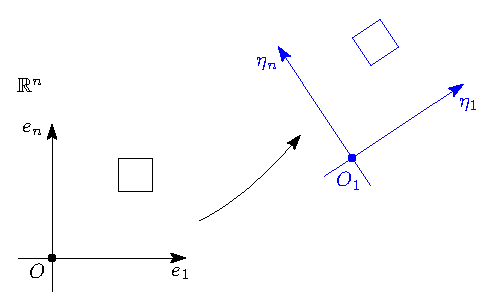
\includegraphics[width=0.35\textwidth]{MA4L12_6.eps}
		\caption{Смена системы координат в $\MR^n$.}
		\label{12_6}
	\end{figure}
	Можно с новой системой координат провести все наши построения и получить меру $\lambda_y$ против первоначальной меры $\lambda_x$. Эти меры совпадают из-за того, что переход от одной системы координат к другой осуществляется преобразованием: $y = Cx + b$, где $C$ - ортогональная матрица. Тогда:
	$$
		 C^*{\cdot}C = C{\cdot}C^* = E \Rightarrow |\det{C}| = 1 \Rightarrow \lambda_y = 1{\cdot}\lambda_x = \lambda_x
	$$
\end{proof}
\begin{rem}
	Пусть $X$ это конечномерное евклидово пространство, $\dim{(X)} = n$. Пусть на $X$ задано скалярное произведение $\inner{\;}{\;}$. Выберем в нём ортонормированный базис: $(e_1, \dotsc, e_n)$ так, что $\inner{e_i}{e_j} = \delta_{ij}$. Тогда:
	$$
		\forall x \in X, \, x = x_1e_1 + \dotsc + x_n e_n \Rightarrow \MU \colon X \to \MR^n, \, \MU(x) = (x_1, \dotsc, x_n)
	$$
	то есть отображение - запись каждой точки $x$ в базисе $(e_1, \dotsc, e_n)$. Кроме того, скалярное произведение будет сохранено:
	$$	
		\inner{\MU(x)}{\MU(y)}_{\MR^n} = \inner{x}{y}_X
	$$
	На $\MR^n$ есть мера Лебега $\lambda$ (только что построили), но тогда на $X$ тоже возникает мера Лебега:
	$$
		\lambda_X(E) = \lambda(\MU(E))
	$$
	Что здесь произвольно? Произвольным является выбор ортонормированного базиса, $\lambda_X$ не зависит от выбора о.н. базиса $e_i$. Тем самым, на всяком конечномерном евклидовом пространстве у нас появляется мера Лебега: вводим произвольно о.н. базис, отождествляем это пространство с $\MR^n$ и оттуда забираем меру Лебега.
	
	Получается мера Лебега это инвариантный объект, если мы совершаем ортогональные преобразования, но она будет зависеть от скалярного произведения: введём на $X$ скалярное произведение по-другому, получим другую меру Лебега.
\end{rem}
\begin{rem}
	Пусть мы в $\MR^n$, где $\inner{x}{y} = x_1 y_1 + \dotsc + x_n y_n$. Возьмем в $\MR^n$ какую-нибудь $k$-мерную аффинную плоскость: $\Pi_k \subset \MR^n$. Выберем в этой плоскости ортонормированный базис: $(\eta_1, \dotsc, \eta_k)$ так, что: 
	$$
		\inner{\eta_i}{\eta_j}_{\MR^n} = \delta_{ij} \Rightarrow \forall p \in \Pi_k, \, p \mapsto (y_1,\dotsc,y_k), \, \exists \, b \colon p = b + \eta_1 y_1 + \dotsc + \eta_k y_k
	$$
	\begin{figure}[H]
		\centering
		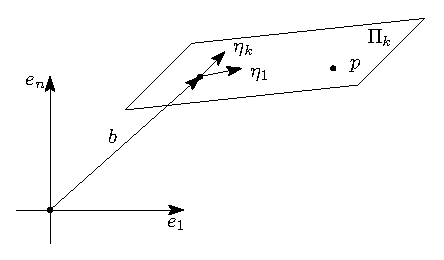
\includegraphics[width=0.35\textwidth]{MA4L12_7.eps}
		\caption{$k$-мерная аффинная плоскость $\Pi_k$.}
		\label{12_7}
	\end{figure}
	Тогда $\Pi_k$ отождествляется с $\MR^k$ $\Rightarrow$ на $\Pi_k$ определена мера Лебега $\lambda_{\Pi_k}$, которая не зависит от выбора прямоугольной системы координат в $\Pi_k$, по тем же причинам, что и выше: пересчет координат будет выдаваться отображением с ортогональной матрицей, чей определитель будет равен $1$. Следовательно в каждой $k$-мерной плоскости в $\MR^n$ у нас появилась своя мера Лебега: $\lambda_{\Pi_k}$.
	
	\textbf{Детальнее}: в $\Pi_k$ мы выбираем систему координат $(\eta_1,\dotsc,\eta_k)$ и получаем координаты $(y_1,\dotsc, y_k)$, следовательно у нас есть взаимнооднозначное отображение $\MU \colon \Pi_k \to \MR^k$. 
	\begin{figure}[H]
		\centering
		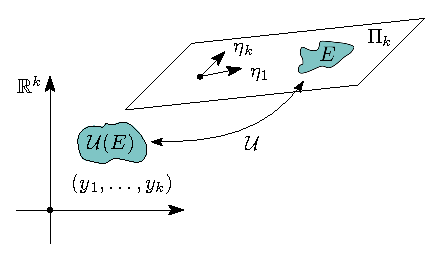
\includegraphics[width=0.4\textwidth]{MA4L12_8.eps}
		\caption{Отождествление $\MR^k$ и $\Pi_k$.}
		\label{12_8}
	\end{figure}
	Тогда всякое множество $E \subset \Pi_k$ переходит в множество $\MU(E)$. В $\MR^k$ мы можем посчитать обычную меру Лебега у этого множества: $\lambda(\MU(E))$ и эту меру Лебега припишем мере множества $E$:
	$$
		\lambda(\MU(E)) = \lambda_{\Pi_k}(E)
	$$
	Если мы вводим другую систему координат: $(z_1,\dotsc, z_k)$, то проделаем для неё всё тоже самое, получив отображение $\wte{\MU}$, тогда:
	$$
		\lambda(\wte{\MU}(E)) = \lambda_{\Pi_k}(E) = \lambda(\MU(E))
	$$
	где равенства верны в силу того, что переход между системами координат задается так:
	$$
		z  = \ML (y)= Cy + b, \, |\det{C}| = 1 \Rightarrow \wte{\MU}(E) = \ML(\MU(E)) \Rightarrow \lambda(\wte{\MU}(E)) = |\det{C}|{\cdot}\lambda(\MU(E)) = \lambda(\MU(E))
	$$
\end{rem}

\begin{theorem}
	$L(x) = Ax + b \colon \MR^k \to \MR^n$, где $n \geq k$ и $\rk{(A)} = k$. Тогда $L(\MR^k) = \Pi_k$ - $k$-мерная аффинная плоскость в $\MR^n$ и верно, что для всякого измеримого ограниченного множества $E \subset \MR^k$:
	$$
		\lambda_{\Pi_k}(L(E)) = \sqrt{\det{(A^T{\cdot}A)}}{\cdot}\lambda(E)
	$$
\end{theorem}
\begin{rem}
	С помощью этой теоремы можно считать объемы в $k$-мерных плоскостях, где мы знаем как эти плоскости были заданы параметрически. На плоскостях ещё можно использовать меру Лебега без каких-либо специальных конструкций, чтобы перейти от плоскостей к кривым поверхностям потребуется вместо меры Лебега рассмотреть меру Хаусдорфа.
\end{rem}

Если в $\MR^k$ мы взяли $(y_1,\dotsc, y_k)$, то смотря обратное отображение к $\MU$, мы задаем плоскость $\Pi_k$ так: 
$$
	y_1\eta_1 + \dotsc + y_k \eta_k + h = Ay + h
$$ 
где $A$ это матрица у которой $\det{(A^T{\cdot}A)} = 1$. В теореме выше предлагается брать не ортонормированные вектора, а произвольные.

\begin{rem}
	Возьмем множества $X, Y$ и какое угодно отображение $f \colon X \to Y$, $\sigma$-алгебру $\MA$ на $X$ и меру $\mu$ на ней. Рассмотрим набор: $\{C \colon f^{-1}(C) \in \MA\}$ это $\sigma$-алгебра:
	$$
		\VN = f^{-1}(\VN), \, Y = f^{-1}(X), \, f^{-1}(\cap_i C_i) = \cap_i f^{-1}(C_i)
	$$
	На этой $\sigma$-алгебре возникает мера: $\mu \circ f^{-1}(C) = \mu(f^{-1}(C))$ и так мы перенесем меру из $X$ с помощью отображения $f$ на $Y$. Заметим, что никаких требований к $f$ здесь нет, но $\sigma$-алгебра на $Y$ может оказаться очень бедной.
\end{rem}

\end{document}